\section{Reinforcement Learning}
The goal of any \emph{reinforcement learning} task is to learn an optimal \emph{policy} \(\pi : S \to A\) that maps the state of the environment to actions so as to maximize the expected \emph{reward}. The agent learns by interacting with the environment. The agent receives a reward $r_t$ and observes the next state $s_{t+1}$ after taking an action $a_t$ in state $s_t$. The agent's goal is to optimize for the \emph{total future discounted reward} which is given by:
\[
    V^\pi(s) = \sum_{t=0}^\infty \gamma^t r_t,\quad 0\leq \gamma < 1
\]
Given an optimal value function $V^*(s)$, the optimal policy $\pi^*(s)$ is given by:
\[
    \pi^*(s) = \text{arg}\max_a \left[r(s,a) + \gamma V^*\left(\delta(s,a)\right)\right]
\]
Many ways to solve this policy optimization problem when all else is know but in unknown environment we must learn \(\delta\) and \(r\).\\
\subsection{Q-Function}
The \emph{Q-function} is a function of the state and action that gives the expected total future discounted reward for taking action $a$ in state $s$ and following policy $\pi$ thereafter. The optimal Q-function is given by:
\[
    Q(s,a) = r(s,a) + \gamma V^*\left(\delta(s,a)\right)
\]
where $r(s,a)$ is the reward for taking action $a$ in state $s$ and $\delta(s,a)$ is the next state after taking action $a$ in state $s$. The optimal policy is given by:
\[
    \pi^*(s) = \text{arg}\max_a Q(s,a)
\]
\subsubsection{Q-Learning}
The learner represents the hypothesis space as a table of Q-values indexed by state and action. The learner interacts with the environment by taking actions and observing the next state and reward. The learner updates the Q-values values in the table using the following update rule:
\[
    \hat{Q}(s_t,a) \gets r + \gamma \max_{a^\prime} \hat{Q}(s_{t+1},a^\prime)
\]
This equation continuously estimates the optimal Q-function by bootstrapping from the current estimate of the optimal Q-function. The learner selects actions using an $\epsilon$-greedy policy. The learner continues to interact with the environment until convergence.
\emph{\textbf{Q-Learning Algorithm:}}
\begin{enumerate}
    \item Initialize Q-values $\hat{Q}(s,a)$ arbitrarily.
    \item Observe current state $s_t$.
    \item Repeat forever:
    \begin{enumerate}
        \item Select action $a_t$ using %$\epsilon$-greedy policy.
        \item Observe reward $r_t$ and next state $s_{t+1}$.
        \item Update Q-values using the update rule. (listed above)
        \item $s_t \gets s_{t+1}$.
    \end{enumerate}
\end{enumerate}
\subsubsection{Exploration:}
The Q-Learning algorithm is ambiguous to the action selection process. The $\epsilon$-greedy policy is a simple way to balance exploration and exploitation. The $\epsilon$-greedy policy selects a random action with probability $\epsilon$ and the greedy action with probability $1-\epsilon$. Another policy allows us to rely on the Q-values to select actions using our trust in Q to determine the probability that we follow Q's hypothesis. \emph{State Transition Updates} during exploration \(\hat{Q}(s,a)\) reward values are only updated when we encounter a non-zero rewaerd.

% \subsubsection{Stochastic Environments:}
% In stochastic environments, the reward and next state are not deterministic. The Q-Learning algorithm can be modified to handle stochastic environments by maximizing the expected Q-value:
% \[
%     \hat{Q}(s_t,a) \gets r + \gamma \mathbb{E}_{a^\prime \sim \pi} \left[\hat{Q}(s_{t+1},a^\prime)\right]
% \]
\begin{center}
    \emph{\textbf{Grid World Example:}}\\
    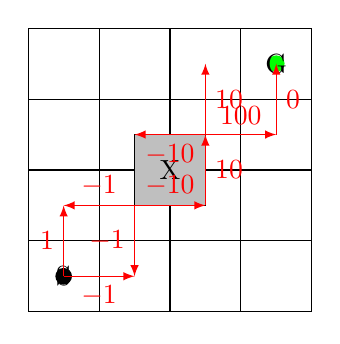
\begin{tikzpicture}[scale=0.9]
        % Draw vertical lines
        \draw (0,0) -- (0,4);
        \draw (1,0) -- (1,4);
        \draw (2,0) -- (2,4);
        \draw (3,0) -- (3,4);
        \draw (4,0) -- (4,4);
        % Draw horizontal lines
        \draw (0,0) -- (4,0);
        \draw (0,1) -- (4,1);
        \draw (0,2) -- (4,2);
        \draw (0,3) -- (4,3);
        \draw (0,4) -- (4,4);
        % Draw start and goal
        \node[circle,fill=black, inner sep=0pt,minimum size=6pt] (start) at (0.5, 0.5) {};
        \node[circle,fill=green, inner sep=0pt,minimum size=6pt] (goal) at (3.5, 3.5) {};
        % Draw obstacles
        \filldraw[fill=gray!50!white, draw=black] (1.5,1.5) rectangle (2.5,2.5);
        % Label cells
        \node at (0.5,0.5) {S};
        \node at (3.5,3.5) {G};
        \node at (2,2) {X};
        % Add Q reward predictions with arrows
        \draw[-latex, red] (0.5,0.5) -- (0.5,1.5) node[midway, left] {$1$};
        \draw[-latex, red] (0.5,0.5) -- (1.5,0.5) node[midway, below] {$-1$};
        \draw[-latex, red] (1.5,1.5) -- (2.5,1.5) node[midway, above] {$-10$};
        \draw[-latex, red] (2.5,1.5) -- (2.5,2.5) node[midway, right] {$10$};
        \draw[-latex, red] (1.5,1.5) -- (1.5,0.5) node[midway, left] {$-1$};
        \draw[-latex, red] (1.5,1.5) -- (0.5,1.5) node[midway, above] {$-1$};
        \draw[-latex, red] (2.5,2.5) -- (3.5,2.5) node[midway, above] {$100$};
        \draw[-latex, red] (3.5,2.5) -- (3.5,3.5) node[midway, right] {$0$};
        \draw[-latex, red] (2.5,2.5) -- (2.5,3.5) node[midway, right] {$10$};
        \draw[-latex, red] (2.5,2.5) -- (1.5,2.5) node[midway, below] {$-10$};
    \end{tikzpicture}
\end{center}





